\documentclass[11pt]{article}

\usepackage[margin=1in]{geometry}
\usepackage{amsmath, amssymb}
\usepackage{graphicx}
\usepackage{float}
\usepackage{booktabs}
\usepackage{xcolor}
\usepackage{array}
\usepackage{tikz}
\usetikzlibrary{positioning,calc}
\usepackage{caption}
\usepackage{url}
\usepackage{hyperref}
\hypersetup{
  hidelinks,
  pdftitle={Offline Diagnostics for Plugin-Based Agent Harnesses: Design, Check Lifecycle, and Field Experience with DeepSeek Harness},
  pdfauthor={moonquake2004}
}

\providecommand{\tightlist}{%
  \setlength{\itemsep}{0pt}\setlength{\parskip}{0pt}}

\title{Offline Diagnostics for Plugin-Based Agent Harnesses: Design, Check
Lifecycle, and Field Experience with DeepSeek Harness}
\author{moonquake2004}
\date{August 15, 2026}

\begin{document}

\maketitle

\begin{abstract}
DeepSeek Harness (dsh) is a plugin-based agent harness whose central
design tenet --- \emph{``everything is a plugin''} --- is realized on
Cordis, a meta-framework of \emph{spatiotemporal composability} [2],
[3]. While the architecture makes every capability (model adapters,
tools, sessions, the agent loop itself) replaceable at configuration
time, it also inherits a systemic fragility: a single malformed patch, a
duplicate entry id, a shadowed module instance, or a corrupted session
log can brick the profile at boot or stall the entire web server with
little or no diagnostics. This paper reports on the design,
implementation, and field experience of \emph{dsh-doctor}, an offline
diagnostic for this failure space, and derives from it a
\emph{check-lifecycle model}: (i) checks as declarative data distributed
through a remote catalog; (ii) introspection of installed harness
contracts instead of hard-coded assumptions; (iii) a fixture-based
certification gate that proves a check does not false-positive and does
catch its target; and (iv) an evolution loop from community report to
certified check. We document 30 checks mapped to 18 community failure
reports, 64 regression tests that have caught real bugs in the tool's
own history, a three-round false-positive elimination campaign, and the
convergence of three independent community tools on a shared
machine-readable contract. We conclude with open problems for the
broader ecosystem: check registry governance, certification matrices
across release trains, and the role of formal composability guarantees
in preventing whole failure classes.

\textbf{Keywords:} agent harness, plugin systems, offline diagnostics,
composability, check lifecycle, DeepSeek Harness, Cordis
\end{abstract}

\section{Introduction}\label{introduction}

Modern AI agent harnesses have moved from monolithic loops to composable
plugin architectures. DeepSeek Harness (dsh) operationalizes
\emph{``everything is a plugin''}: model adapters, tool registries,
session storage, sandboxing, the agent loop, and even the web UI are all
plugins composed at runtime by Cordis, a plugin framework formalized in
an 88-page paper on \emph{spatiotemporal composability} [2]. The dsh
repository has attracted over 110,000 stars and 10,000 forks within days
of its public release [1], and a community ecosystem of plugins and
marketplaces is forming around it at high velocity.

This architectural bet carries a distinctive failure mode. In a harness
where configuration replaces code as the composition mechanism, the
\emph{deployment-time} state --- profile manifests, bundle patches, the
composed plugin tree, the append-only session logs --- becomes the
primary locus of fragility. Empirically, this is not hypothetical: the
community has reported a recurring family of failures in which a single
bad install bricks the profile at boot, stalls tool execution, or makes
sessions unrecoverable, often with opaque errors that point at nothing
actionable [7], [8], [11], [13], [17], [18],
[19]. The harness's own \texttt{-\/-dump-config} never mounts the
loader, so it passes on broken setups; the failure class was
consolidated into an advisory, \emph{``the plugin-install path needs
guardrails''} [6].

This paper makes the following contributions:

\begin{enumerate}
\def\labelenumi{\arabic{enumi}.}
\item
  \textbf{A taxonomy and empirical corpus.} We consolidate 18 community
  failure reports into a three-group taxonomy (environment,
  profile/composition, session-log integrity), each entry verified
  against the vendored harness source and, where possible, reproduced
  with synthetic fixtures.
\item
  \textbf{The design of dsh-doctor.} A zero-dependency, single-file
  offline diagnostic that runs before boot and reports which of the
  known failure classes will bite, as a CLI and as a dsh plugin with a
  settings panel and a read-only JSON API.
\item
  \textbf{A remote check catalog (checks-as-data).} New checks are
  declarative rules shipped as data and distributed without a plugin
  release, with a security model that guarantees the remote payload can
  never execute code.
\item
  \textbf{A check-lifecycle model.} We argue that checks themselves rot
  as the harness evolves, and propose four properties ---
  checks-as-data, introspection, a fixture-based certification gate, and
  an evolution loop --- each backed by a running reference
  implementation.
\item
  \textbf{Field experience.} We document 30 checks, 64 regression tests,
  real bugs the corpus caught in the tool's own history, a three-round
  false-positive elimination campaign, and the convergence of three
  independent community tools on a shared \texttt{dsh-doctor/v1} output
  contract.
\end{enumerate}

The remainder of this paper is organized as follows. Section 2 provides
background on the harness architecture and the threat model. Section 3
surveys related work. Section 4 details the system design. Section 5
presents the check-lifecycle model. Section 6 evaluates the approach
empirically. Section 7 discusses limitations and open problems. Section
8 concludes.

\section{Background and Threat
Model}\label{background-and-threat-model}

\subsection{DeepSeek Harness and
Cordis}\label{deepseek-harness-and-cordis}

DeepSeek Harness is an open-source (MIT) agent harness whose products
--- web app, headless runner --- are composed entirely from plugins
[1], [4]. The composition framework is Cordis [3], which the
harness \emph{source-vendors} into its own repository under the scope
\texttt{@deepseek-ai/cordis} (version 4.0.1, based on upstream
4.0.0-rc.7, with local hardening patches) [4], [24]. Cordis's
model fits in five ideas: plugins as objects contributing capabilities;
a context as a store of named capabilities; declared rather than ordered
dependencies; typed events with declared dispatch; and teardown ---
every registration knows how to undo itself [24], [25]. The
formal foundation [2] lifts classical effect/coeffect concepts to
runtime mechanisms: \emph{revertible effects} (every context
transformation carries a tracked inverse) and \emph{reactive coeffects}
(context changes notify components), unified into a single context type;
the calculus establishes spatiotemporal composability from a single
component to interleaved systems.

In implementation, a \emph{Fiber} is the per-instance lifecycle state
machine of a plugin (PENDING  $\to$  LOADING  $\to$  ACTIVE  $\to$  FAILED  $\to$  DISPOSED  $\to$ 
UNLOADING); a plugin that declares \texttt{inject} dependencies waits in
PENDING until they are resolvable [2], [24].
\texttt{ctx.effect(fn)} registers a side effect with a disposer;
\texttt{ctx.provide} and \texttt{ctx.on} build on it. Two properties
matter for our threat model:

\begin{itemize}
\item
  \textbf{Declared dependencies are not enforced at the OS level.}
  \texttt{inject} constrains what a plugin can \emph{see} through the
  context, not what the process can do; a plugin that fails to declare a
  dependency may nonetheless activate before the service is ready (or
  never, if the service never appears in its scope), producing either a
  permanent PENDING or an undefined-service crash [17], [19].
\item
  \textbf{Composition is configuration.} The composed tree is decided by
  profiles, bundles, and patches --- text files that any install path
  can corrupt or duplicate [4], [13], [19].
\end{itemize}

\subsection{Profiles, Bundles, and
Patches}\label{profiles-bundles-and-patches}

The harness defines three configuration layers [4]:

\begin{itemize}
\tightlist
\item
  \textbf{Bundle} --- distributes a set of Cordis configuration and the
  plugin code that mounts them, declared via \texttt{dsh.bundle.patch}
  in the package manifest.
\item
  \textbf{Profile} --- a named composition listing which bundles to
  stack (web and headless ship as templates), stored under the harness
  home
  (\texttt{~/.dsh/profiles/\textless{}name\textgreater{}}).
\item
  \textbf{Patch} --- replaces or inserts configuration rows, applied in
  order: bundles (in declaration order)  $\to$  profile
  \texttt{cordis.patch.yml}  $\to$  home-level patch  $\to$  CLI \texttt{-\/-patch}
  overlay. A patch locates an entry by id and replaces its whole config,
  or inserts a new row.
\end{itemize}

Because ``the last layer wins'' and rows are keyed by id,
\textbf{duplicate ids across layers are a hard boot failure}: the
loader's \texttt{EntryGroup.update} throws
\texttt{duplicate\ loader\ entry\ id} [7], [19]. This is the
first and most frequently reported crash class.

\subsection{Append-Only Session
Logs}\label{append-only-session-logs}

A session is an append-only event log (typically
\texttt{session.jsonl.zstd}) with monotonically increasing \texttt{seq}
values; the model reads a \emph{projection} of the log, and the
invariant \emph{``model-visible means logged''} guarantees everything
the model sees can be reconstructed from the log [4], [24],
[25]. The log is also the source for resume, fork, audit, and token
metering. Threats to log integrity include: \texttt{seq\ ==\ index} gaps
and duplicates [9]; post-\texttt{end-seed} replay of a committed
tail [12]; unknown event types without \texttt{ignorable} causing
wholesale refusal [14]; single-frame zstd containers that make
\texttt{session.list} fail wholesale [16]; and
\texttt{sourceEventSeqs} referencing non-earlier events after compaction
[15].

\subsection{Threat Model}\label{threat-model}

We define the diagnostic target as \emph{deployment-time state}:
environment (PATH, node version, native binaries, storage, ports),
profile composition (manifests, patches, resolved bundles), and session
logs (structure, continuity, integrity). The diagnostic must run
\textbf{offline} (before boot, when the harness itself may be unusable),
be \textbf{zero-dependency} (no harness internals required), and produce
\textbf{actionable} output (what to fix, not just that something is
wrong). Attacks or accidents are out of scope for prevention; the tool's
contract is detection and remediation guidance.

\section{Related Work}\label{related-work}

\subsection{Plugin-System
Fragility}\label{plugin-system-fragility}

Plugin systems have long traded composability for deployment fragility.
VS Code's extension host, for example, defers full uninstall cleanup of
executable extensions to process restart, a pattern the Cordis paper
explicitly cites as motivation for component-level revertible effects
[2]. Koishi [5], the chatbot framework that predates and uses
Cordis, demonstrates the same composition model at scale but in a
community where plugin authors control their own installs. The
distinctive property of the dsh ecosystem is that \emph{the harness
itself is assembled from plugins}, so composition failures are boot
failures, not feature degradations.

\subsection{Offline Diagnostics for Developer
Tooling}\label{offline-diagnostics-for-developer-tooling}

Offline/static diagnostics are well established in compiler and
package-manager tooling (e.g., \texttt{npm\ doctor},
\texttt{cargo\ doctor}, IDE linters). What is novel here is the
\emph{object} of diagnosis: not source code or dependency graphs, but a
composed runtime tree whose contracts (event-type tables, module
symbols, patch grammar) live in an installed, versioned artifact. The
closest analog is runtime anchor verification, which we develop further
in Section 5.

\subsection{The Emerging dsh Diagnostic
Ecosystem}\label{the-emerging-dsh-diagnostic-ecosystem}

Within weeks of the harness release, several independent diagnostic
tools appeared: dsh-plugin-doctor (author-side pre-publish checks,
\texttt{profile-shadow} tripwire) [21]; dsh-diagnose (symptom-based
diagnosis with release-anchored knowledge) [22]; ciceroyang's
zero-dependency CLI [30]; boyin111-1's sibling offline diagnostic
[31]; plus session-focused tools (dsh-session-doctor,
dsh-session-repair). A proposal for an official \texttt{dsh\ doctor}
command and a community registry contract has been consolidated in
[20], and a broader RFC covering registry v2,
\texttt{dsh\ plugin\ check}, and \texttt{dsh\ doctor} in [32]. This
paper's contribution is distinct: the \emph{check-lifecycle} layer
underneath all of these --- how any check, in any of these tools, is
born, proven correct, distributed, and kept honest across harness
upgrades [33].

\subsection{Formal Foundations}\label{formal-foundations}

The Cordis paper [2] provides the theoretical backing for the
harness's composition semantics and, we argue in Section 5, for the
\emph{diagnostic} layer as well: the same failure to achieve revertible
effects and reactive coeffects that the paper formalizes is what
manifests in the field as leaked registrations [10], [11] and
silent contract drift [8].

\section{System Design:
dsh-doctor}\label{system-design-dsh-doctor}

\subsection{Architecture}\label{architecture}

dsh-doctor is a single-file, zero-dependency Node.js program (currently
\textasciitilde1,050 lines) that also ships as a proper dsh plugin: the
plugin's server route shells out to the same CLI with \texttt{-\/-json},
so the CLI, the settings panel, and the HTTP API
(\texttt{GET\ /dsh-doctor/run}) share one source of truth [26]. The
repo-root entry is a thin wrapper for \texttt{node\ dsh-doctor.mjs}
compatibility.

\begin{figure}[H]
\centering
\resizebox{\textwidth}{!}{%
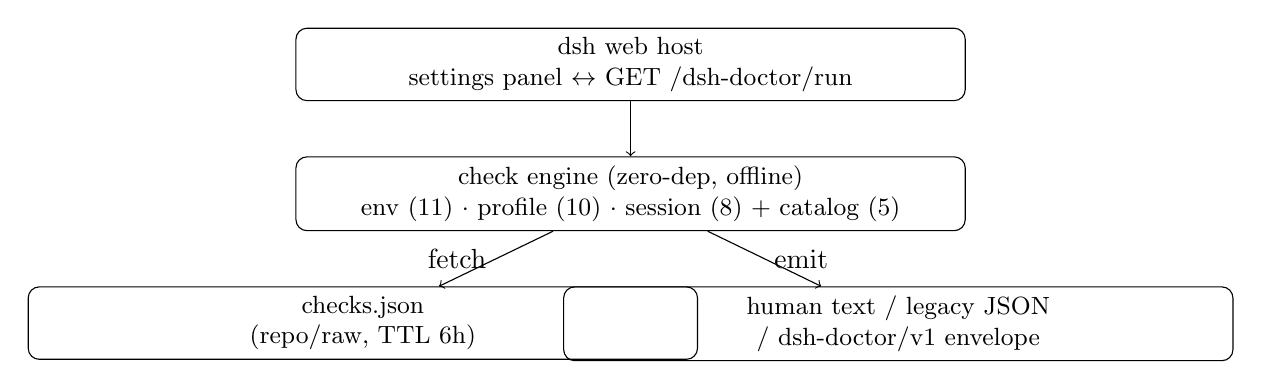
\begin{tikzpicture}[node distance=1.1cm, box/.style={draw, rounded corners, align=center, font=\small, minimum width=8.5cm}]
\node[box] (host) {dsh web host\\ settings panel $\leftrightarrow$ GET /dsh-doctor/run};
\node[box, below=0.7cm of host] (engine) {check engine (zero-dep, offline)\\ env (11) $\cdot$ profile (10) $\cdot$ session (8) + catalog (5)};
\node[box, below=0.7cm of engine, xshift=-3.4cm] (catalog) {checks.json\\ (repo/raw, TTL 6h)};
\node[box, below=0.7cm of engine, xshift=3.4cm] (out) {human text / legacy JSON\\ / dsh-doctor/v1 envelope};
\draw[->] (host) -- (engine);
\draw[->] (engine) -- (catalog) node[midway, left] {fetch};
\draw[->] (engine) -- (out) node[midway, right] {emit};
\end{tikzpicture}
}
\caption{dsh-doctor architecture: one check engine, three output modes, remote catalog with TTL cache.}
\label{fig:arch}
\end{figure}

The tool runs three groups of checks --- \texttt{env}, \texttt{profile},
\texttt{session} --- plus a remote catalog layer, and emits either
human-readable output or machine-readable JSON. Exit codes: \texttt{0}
all pass, \texttt{1} problems found (or any WARN in envelope mode),
\texttt{2} any FAIL in envelope mode.

\subsection{The 30 Checks}\label{the-30-checks}

As of this writing the tool ships 25 built-in checks and 5 catalog
checks (Section 4.3), each mapped to one or more community failure
reports:

\textbf{Environment (7 built-in + 4 catalog):} E1 binaries on PATH
(\texttt{node}/\texttt{pnpm}/\texttt{zstd}) [\#1270]; E2
\texttt{.env} is a file not a directory [\#71]; E3 node version and
\texttt{-\/-expose-internals} reachability [\#113], [\#1313]; E4
node-pty native binary presence [\#1219]; E5 storage JSON validity
(strict UTF-8 + parse) [\#1357]; E6 \textbf{anchor tripwire} ---
verifies the contracts our S6/S7/S10 checks rely on still exist in the
installed \texttt{dsh-session} [9]; E10 web port 3080 availability
(dsh web itself = normal, foreign process = FAIL) [\#1719] [20];
E7 \texttt{dsh} on PATH (catalog); E8 profile \texttt{.npmrc} workspace
flag (catalog, warn) [23]; E9 \texttt{config/workspace.json}
validity (catalog) [\#1357]; E11 \texttt{settings.yaml} writability
/ sudo ownership (catalog) [34].

\textbf{Profile (10 built-in):} P1 bundle resolution
[\#917]/[\#1377]/[\#880]; P2 bundle-vs-user-patch insert id
collisions (the \texttt{duplicate\ loader\ entry\ id} crash)
[\#1404] [7]; P3 user-patch insert names resolvable from the
profile anchor [\#1197]/[\#880]; P4 \texttt{file:} dependencies
intact [\#1197]; P5 top-level \texttt{@deepseek-ai/*} duplication
(dual module instances) [\#1486] [8]; P7
\texttt{cordis.patch.yml} structural lint
(\texttt{~\ insert:} null literal, tab indentation,
missing colon, top-level mapping+sequence mixing) [\#1724] [13];
P8 adapter-provider registration conflicts (\texttt{DUPLICATE\_ADAPTER})
[\#1904] [35]; P9 \texttt{ctx.settings} usage without declared
settings dependency [\#1904] [35]; P10 inject referencing
client-only services (\texttt{@deepseek-ai/dsh-client-*})  $\to$  permanent
PENDING [\#1947] [17]; P11 installed bundle's \texttt{main}
entry artifact missing (unbuilt source tree) [\#1965] [18].

\textbf{Session (8 built-in):} S1 orphan \texttt{tool\_call}
[\#1363]/[\#1544]; S2 unclosed turns [\#466]/[\#1265];
S6 \texttt{seq\ ==\ index} continuity with chunk expansion
[\#1333]/[\#1452]/[\#1469]; S7 post-\texttt{end-seed} replay
[\#1497]; S8 unknown event types without \texttt{ignorable}
[\#1538]; S9 zstd container frame count [\#1043]; S10
\texttt{sourceEventSeqs} drift [\#1469]; S11 whole-session scan:
corrupt  $\to$  quarantine, oversized  $\to$  cold-start heap risk [\#1550].

Each built-in check is validated by at least one synthetic fixture
asserting isolation: on a \emph{bad} fixture the target check must fail
while every other check passes, and healthy baselines must not
false-positive. This discipline is what makes the corpus useful for the
certification model of Section 5.

\textbf{Table 1 --- Check inventory (30 checks, 18 mapped community
reports, as of v0.2.7).}

\begin{table}[H]
\centering
\caption{Check inventory (30 checks, 18 mapped community reports, v0.2.7).}
\label{tab:checks}
\resizebox{\textwidth}{!}{%
\begin{tabular}{@{}llllp{6.2cm}@{}}
\toprule
Group & IDs & Count & Coverage class & Representative reports\\
\midrule
env (built-in) & E1--E6, E10 & 7 & PATH / files / native binary / storage / anchors / port & [\#1270] [\#71] [\#113] [\#1219] [\#1357] [\#1534] [\#1719]\\
env (catalog) & E7--E9, E11 & 4 & declarative probes (path/JSON/text/writable) & [\#1270] [23] [\#1357] [34]\\
profile & P1--P5, P7--P11 & 10 & composition: resolution / collisions / patch syntax / dual-instance / inject semantics / artifacts & [\#1404] [\#1486] [\#1697] [\#1724] [\#1904] [\#1947] [\#1965]\\
session & S1, S2, S6--S11 & 8 & log integrity: continuity / replay / types / containers / drift / heap & [\#1363] [\#466] [\#1333] [\#1497] [\#1538] [\#1043] [\#1469] [\#1550]\\
\bottomrule
\end{tabular}
}
\end{table}

Coverage honesty: two symptom families (sandbox denials, approval
policy) have \textbf{no} offline probe and are explicitly documented as
gaps in the published symptom $\to$ check mapping [26], [34].

\subsection{Layer A: Remote Check Catalog
(Checks-as-Data)}\label{layer-a-remote-check-catalog-checks-as-data}

The catalog (\texttt{plugin/checks.json}) holds declarative rules ---
data, not code. The engine executes only read-only probe primitives
(\texttt{command-exists},
\texttt{path-exists}/\texttt{is-dir}/\texttt{is-file},
\texttt{json-valid}, \texttt{text-contains}/\texttt{text-not-contains},
\texttt{file-size-above}, \texttt{glob-count}, \texttt{file-writable}),
so a remote payload can never execute code; it can only add pattern
checks. Each run fetches the catalog from the repository (3 s timeout),
caches it under the harness home (TTL 6 h), and falls back to the
last-known-good cache, then the bundled copy. New checks therefore reach
every installed instance within  $\leq$ 6 h of being committed upstream, with
\textbf{zero plugin releases} --- five catalog checks have shipped this
way to date. This property (Section 5, property 1) is the distribution
mechanism that makes the ecosystem's check inventory updateable without
the ``update the tool'' tax.

\subsection{Layer B: Self-Update}\label{layer-b-self-update}

The tool also watches its own npm version (\texttt{dist-tags.latest}
vs.~installed), with the same TTL/fallback discipline. It never touches
the installation unasked: \texttt{-\/-update} runs
\texttt{pnpm\ install} in the hosting profile,
\texttt{DSH\_DOCTOR\_AUTO\_UPDATE=1} enables opt-in automatic updates,
and an honest boundary is documented --- Cordis loads plugins at boot,
so the new engine activates only after a restart.

\subsection{Output Contract: \texttt{dsh-doctor/v1} Envelope}\label{output-contract-dsh-doctorv1-envelope}

To make diagnostics consumable by other tools (CI, marketplaces, symptom
tools), dsh-doctor emits --- alongside its legacy JSON --- a v1 envelope
[27]:

\begin{verbatim}
{
  "schema": "dsh-doctor/v1",
  "tool": "dsh-doctor",
  "generatedAt": "ISO-8601",
  "profile": "<name or dir>",
  "exitCode": 0,
  "summary": { "pass": 2, "warn": 0, "fail": 0 },
  "ok": true,
  "checks": [ { "name": "<check id>", "status": "pass", "detail": "..." } ]
}
\end{verbatim}


with lowercase \texttt{pass\textbar{}warn\textbar{}fail} status
vocabulary, exit codes \texttt{0/1/2} (all-pass / any-WARN / any-FAIL),
and a documented minimal compatible subset
\texttt{\{ok,\ checks:[\{name,status,detail\}]\}} that any consumer
of the full envelope can read [27]. Two other community tools have
adopted this contract (Section 6.4).

\section{The Check-Lifecycle
Model}\label{the-check-lifecycle-model}

The RFC consolidating the ecosystem's tooling [32] standardizes the
\emph{tools}: registry contract, publish gate, doctor command. What
remains unspecified is the \textbf{lifecycle of the checks themselves}.
We argue this is a first-class problem, because checks rot --- and
false-positive.

\textbf{Checks rot.} Every check encodes assumptions about harness
internals: event-type tables, seq semantics, patch grammar, file layout,
module symbols. Every harness release can silently invalidate them.
Field evidence: the anchor-tripwire check E6 exists \emph{precisely}
because of this; the dual-module-instance crashes
[\#1486]/[\#1697] [8], [11] and the process-singleton
collision [\#1415] [10] were contract-drift failures no static
list caught early; and our own P3 shipped silently dead for months --- a
wrong regex matched nothing, so it always ``passed'' --- until fixture
testing exposed it (Section 6.1).

\textbf{Checks false-positive.} Static checks without semantic
boundaries misfire: a substring match on \texttt{npm\ run} misfires on
\texttt{pnpm\ run} [13]; a name match on \texttt{exec} misfires on
\texttt{node:sqlite}'s \texttt{DatabaseSync.exec} [36]; three rounds
of P9 false positives were eliminated in this work (Section 6.2). A
noisy check poisons the credibility of the entire tool --- worse than no
check.

We therefore propose four properties, each backed by a running reference
implementation in dsh-doctor:

\textbf{Property 1 --- Checks are data, not code.} A check is a
declarative, read-only probe definition plus its target contract anchor,
its good/bad fixture pair, and the release train it was certified on.
Distribution happens through a \emph{check registry} (not a plugin
registry) with TTL cache and offline fallback. \emph{Reference:} the
Layer-A catalog (Section 4.3), which has shipped 5 checks with zero
releases.

\textbf{Property 2 --- Introspection instead of hardcoding.} Read the
installed harness's contracts (event-type table, module symbols, patch
grammar) to derive or validate expectations. On upgrade, either the
anchor passes (check still valid) or the tripwire fails loudly (no
silent rot). \emph{Reference:} S8 parses the installed
\texttt{KNOWN\_SESSION\_EVENT\_TYPES} with fallback; E6 verifies
\texttt{expandRow}/\texttt{session/end-seed}/\texttt{sourceEventSeqs}
still exist in the installed \texttt{dsh-session}. The same idea appears
independently in the knowledge domain as dsh-diagnose's
\texttt{check-knowledge-anchors} [22].

\textbf{Property 3 --- Certification gate.} A check enters the ecosystem
only if its fixture pair proves \emph{good-does-not-false-positive,
bad-gets-caught} on the declared train. This upgrades shape-level
contract checks to \emph{correctness-level} certification.
\emph{Reference:} the 64-test corpus whose isolation property has caught
real bugs (Section 6.1), and the fixture-based acceptance harness
proposed in [32].

\textbf{Property 4 --- Evolution loop.} Community report  $\to$  candidate
check  $\to$  fixture certification  $\to$  catalog distribution  $\to$  auto-update. The
diagnostic layer itself ``evolves on the fly'' --- the paper's theme
[2] applied to the diagnostics. \emph{Reference:} the report-driven
addition of P8--P11 (Section 6.1) plus the Layer-B update mechanism.

We also propose a check-entry schema:

\begin{verbatim}
{
  "id": "E11-settings-writable",
  "section": "env",
  "severity": "error",
  "probe": { "type": "file-writable", "path": "{home}/settings.yaml", "required": false },
  "anchor": { "package": "@deepseek-ai/dsh-settings", "symbol": null, "train": "0.1.0-rc.6" },
  "fixtures": { "good": "path-or-inline", "bad": "path-or-inline" },
  "certifiedOn": "0.1.0-rc.6"
}
\end{verbatim}


A working draft of this model is published as [33].

\begin{figure}[H]
\centering
\resizebox{\textwidth}{!}{%
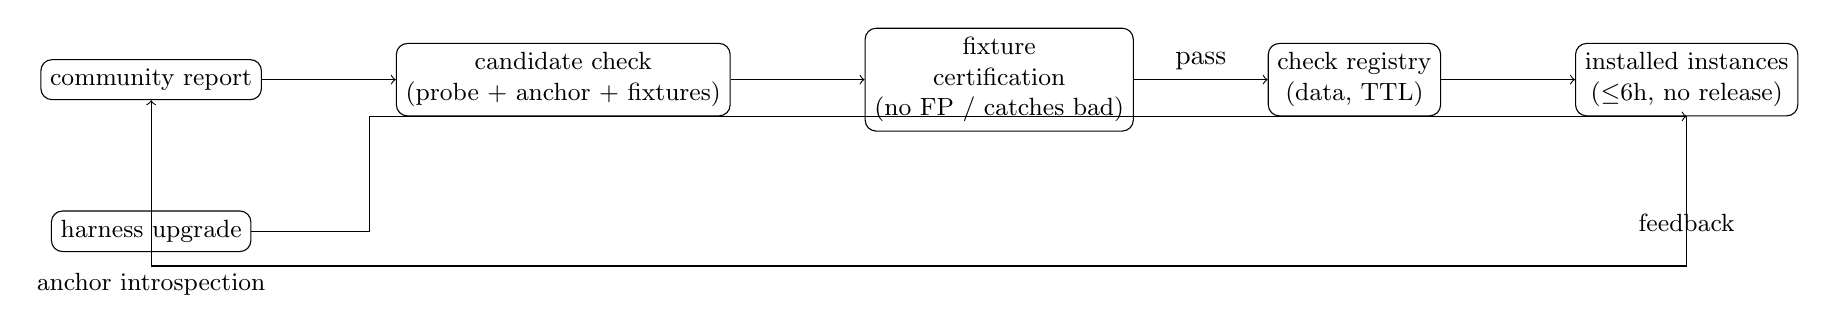
\begin{tikzpicture}[node distance=1.6cm, box/.style={draw, rounded corners, align=center, font=\small}]
\node[box] (report) {community report};
\node[box, right=1.7cm of report] (cand) {candidate check\\ (probe + anchor + fixtures)};
\node[box, right=1.7cm of cand] (cert) {fixture\\ certification\\ (no FP / catches bad)};
\node[box, right=1.7cm of cert] (reg) {check registry\\ (data, TTL)};
\node[box, right=1.7cm of reg] (inst) {installed instances\\ ($\le$6h, no release)};
\node[box, below=1.4cm of report] (up) {harness upgrade};
\draw[->] (report) -- (cand);
\draw[->] (cand) -- (cert);
\draw[->] (cert) -- node[above] {pass} (reg);
\draw[->] (reg) -- (inst);
\draw[->] (inst.south) -- ++(0,-1.9) -| (report.south);
\node[font=\small] at ($(inst.south)+(0,-1.35)$) {feedback};
\draw[->] (up.east) -- ++(1.5,0) |- (inst.south);
\node[font=\small, below=0.15cm of up] {anchor introspection};
\end{tikzpicture}
}
\caption{The check lifecycle: report $\rightarrow$ candidate $\rightarrow$ certify $\rightarrow$ distribute $\rightarrow$ verify (property 4), with introspection (property 2) guarding every upgrade.}
\label{fig:lifecycle}
\end{figure}

\section{Empirical Evaluation}\label{empirical-evaluation}

\subsection{Detection: Real Bugs Caught by the
Corpus}\label{detection-real-bugs-caught-by-the-corpus}

The fixture corpus has repeatedly caught real defects:

\begin{itemize}
\tightlist
\item
  \textbf{P3 silent no-op.} The original regex for user-patch insert
  names matched a patch format that does not exist in the wild (the real
  format indents \texttt{name:} under \texttt{-\ id:} without a dash).
  The check ``passed'' for months without ever checking anything; a
  fixture built from the real format exposed it.
\item
  \textbf{P6 regex overmatch.} The \texttt{text-not-contains} probe's
  pattern let \texttt{\textbackslash{}s} consume the separator space, so
  any \texttt{name:} line matched --- flagging every plugin. Semantic
  correction (\texttt{[\^{}'"\textbackslash{}s]+}
  first, then an internal space) fixed it.
\item
  \textbf{P8--P11 genesis.} All four profile checks were added in
  response to \emph{reported} failures: adapter-provider conflicts
  [\#1904], missing \texttt{settings} inject [\#1904],
  client-only service injects [\#1947], and unbuilt \texttt{main}
  artifacts [\#1965]. Each addition was itself validated by new
  fixtures (now 64 total).
\item
  \textbf{Field validation.} A user's independent fix of a duplicate-id
  boot crash [19] turned out to match P2's exact detection shape,
  and a genuine \texttt{ctx.settings}-without-inject defect was
  confirmed in the same thread --- validating both P2 and P9 against
  real incidents.
\end{itemize}

\subsection{False-Positive Elimination: Three Rounds on One
Check}\label{false-positive-elimination-three-rounds-on-one-check}

P9 (missing \texttt{settings} dependency) was flagged on the author's
own production profile against three plugins. Manual source verification
showed all three were false positives, each a distinct class:

\begin{enumerate}
\def\labelenumi{\arabic{enumi}.}
\tightlist
\item
  \textbf{Substring collision.} \texttt{sctx.settings} (a different
  variable) contains \texttt{ctx.settings} as a substring --- the same
  trap as the \texttt{npm\ run}  $\subseteq$  \texttt{pnpm\ run} substring miscount
  we made while verifying the harness repo's own package.json
  (discussion \#1702, a correction we later acknowledged publicly).
\item
  \textbf{Wrong artifact scope.} A client-side bundle
  (\texttt{client.js}) was being scanned as server code.
\item
  \textbf{Wrong declaration.} \texttt{String.match} returned the
  \emph{first} \texttt{inject\ =\ [...]} array in a bundled file ---
  an internal module's declaration --- masking the plugin's own
  \texttt{inject} (which correctly included \texttt{settings}).
\end{enumerate}

Each was fixed with a targeted mechanism (negative lookbehind; excluding
\texttt{client}/\texttt{web} directories; collecting all inject
declarations and satisfying on any). The same lesson ---
\emph{name-based static checks need semantic boundaries} --- is echoed
by the ecosystem's \texttt{DatabaseSync.exec} false-positive report
[36].

\subsection{Real-Profile Findings}\label{real-profile-findings}

On the author's production profile, the tool reports a clean bill for
all 30 checks. Notably, the same profile \emph{does} carry plugins that
use \texttt{ctx.inject(["settings"],\ cb)} (the safe runtime
pattern), which the final P9 correctly recognizes --- validating that
the check distinguishes the safe pattern from the defective one
[19].

\subsection{Ecosystem Convergence}\label{ecosystem-convergence}

Three independent community tools --- dsh-plugin-doctor [21],
dsh-diagnose [22], and dsh-doctor --- converged on the
\texttt{dsh-doctor/v1} envelope: lowercase status,
\texttt{\{ok,\ checks:[\{name,status,detail\}]\}} minimal subset,
and a provenance \texttt{tool} field. A symptom $\to$ check mapping (16
symptom families  $\leftrightarrow$  our 30 checks, with honest coverage marks including
two documented gaps: sandbox denials and approval policy have no offline
probe) is published in the dsh-doctor README [26], and a contract
document pins the shape [27]. This convergence was driven by
discussion threads [20], [32], [34] and is the concrete
evidence that a shared contract can absorb independently built tools.

\textbf{Table 2 --- Independent diagnostic tools converging on the
\texttt{dsh-doctor/v1} contract.}

\begin{table}[H]
\centering
\caption{Independent diagnostic tools converging on the \texttt{dsh-doctor/v1} contract.}
\label{tab:tools}
\resizebox{\textwidth}{!}{%
\begin{tabular}{@{}lllll@{}}
\toprule
Tool & Side & Checks & Envelope mode & Status vocabulary\\
\midrule
dsh-doctor [26] & user (env/profile/session) & 30 (25 built-in + 5 catalog) & \texttt{--json --envelope} & lowercase pass/warn/fail\\
dsh-plugin-doctor [21] & author (pre-publish) + profile tripwire & manifest/patch/entry/files/build/pack/install/profile-shadow & v1.6.0 \texttt{--profile --json} & lowercase pass/warn/fail\\
dsh-diagnose [22] & user (symptom, knowledge-anchored) & 17 \texttt{dsh-symptom.*} families & \texttt{--doctor-json} & lowercase (adopted)\\
\bottomrule
\end{tabular}
}
\end{table}

\section{Discussion and Open
Problems}\label{discussion-and-open-problems}

\subsection{Threats to Validity}\label{threats-to-validity}

\textbf{Construct validity.} The check inventory and failure taxonomy
were induced from 18 community reports plus the tool's own field
history; both are subject to selection bias (reports that reached the
discussion forum, not the full population of incidents). The ``30
checks'' count is a snapshot (v0.2.7) and grows as new reports arrive
--- we treat the inventory as data (Property 1), not as a fixed
benchmark.

\textbf{Internal validity.} The fixture corpus is single-developer and
synthetic: the good/bad fixtures encode the author's interpretation of
each failure class. Two mitigations: (i) the isolation property (target
fails, others pass) is machine-checked in CI; (ii) several fixtures were
cross-verified against independent implementations (boyin111-1's sibling
tool, dsh-plugin-doctor's acceptance harness [32]).
Cross-implementation fixture sharing remains partial.

\textbf{External validity.} dsh-doctor is evaluated on one harness
(DeepSeek Harness 0.1.0-rc.6 train) and one production profile. The
check-lifecycle \emph{model} (Section 5) is claimed as general, but its
evidence base is a single ecosystem; generalization to other
plugin-based harnesses (e.g., Koishi [5]) is untested. The
environment checks are partially platform-dependent (verified on macOS;
Windows-specific paths exercised only through reported cases
[\#1724], [\#1965]).

\textbf{Conclusion validity.} The empirical claims are case-based
(Section 6): real bugs caught and false positives eliminated are
documented incidents, not randomized trials. We report precision/recall
as open work rather than over-claiming them.

\subsection{Reproducibility}\label{reproducibility}

\begin{itemize}
\tightlist
\item
  \textbf{Artifact:} the tool and all fixtures are in [26]; the
  paper's claims map to the fixed commit \texttt{189f3e2} of
  \texttt{moonquake2004/dsh-doctor}.
\item
  \textbf{Regression suite:} \texttt{node\ -\/-test\ plugin/test/} (64
  tests: 39 fixtures + 25 catalog) reproduces Section 6.1's detection
  cases and the Section 6.2 false-positive eliminations.
\item
  \textbf{Contract:} \texttt{docs/doctor-contract.md} [27] pins the
  envelope; \texttt{docs/check-lifecycle.md} [28] pins the model;
  \texttt{docs/paper-offline-diagnostics.md} is this paper.
\item
  \textbf{Environment:} Node  $\geq$ 18 (tested on 22), pnpm 9.15.9,
  macOS/Windows reports from the cited discussions.
\end{itemize}

\subsection{Open Problems}\label{open-problems}

\textbf{Limitations.} The checks are heuristic and name/regex-based;
they detect \emph{symptoms} (e.g., an inject list naming a client
service) not \emph{proofs}. Semantic boundaries reduce but cannot
eliminate false positives; the certification gate (Property 3) is the
only honest mitigation. Two documented coverage gaps --- sandbox denials
and approval policy --- are runtime-only phenomena with no offline
static probe, and we deliberately do not claim coverage there. The
corpus is single-developer; cross-implementation fixture sharing (with
boyin111-1's sibling tool, for example) is ongoing.

\textbf{The AI-generated plugin problem.} A recurring theme in the
reports is that harness agents themselves generate broken plugins
(missing injects, client services as server dependencies, duplicate
inserts) [17], [19]. This shifts the burden from ``author
discipline'' to ``automated authoring must be checked'' --- making
offline diagnostics a \emph{hard dependency} of the self-evolving-agent
vision, and giving the check-lifecycle model an immediate consumer.

\textbf{Open problems.}

\begin{enumerate}
\def\labelenumi{\arabic{enumi}.}
\tightlist
\item
  \textbf{Check registry governance.} Who hosts the shared check
  registry, and how do canonical ids coexist with tool-local ids
  (currently handled by the \texttt{tool} provenance field)? The
  registry-contract RFC [32] is the natural home, but checks-as-data
  (Property 1) needs a registry of its own.
\item
  \textbf{Certification matrix.} On which release trains must a fixture
  pair pass --- latest only, or N-1 as well? This interacts directly
  with Property 2's introspection: an anchor that passes on the current
  train is the strongest form of ``still certified''.
\item
  \textbf{Signability.} Is pinned-repository-plus-read-only-probes
  sufficient trust for a remote catalog, or do rules need signing?
\item
  \textbf{Formal prevention.} The Cordis paper's revertible effects and
  reactive coeffects [2] could, if fully realized, prevent whole
  failure classes (idempotent \texttt{register()}, host-first
  resolution) --- the diagnostic layer exists today precisely because
  those guarantees are not yet there. We see Property 2 (introspection)
  as the bridge: a check that asserts a \emph{contract} rather than a
  \emph{value} is a runtime-verifiable claim about the harness's own
  composability guarantees.
\end{enumerate}

\section{Conclusion}\label{conclusion}

We presented the design and field experience of dsh-doctor, an offline
diagnostic for a plugin-based agent harness, and generalized from it a
check-lifecycle model. The model's four properties --- checks-as-data,
introspection, fixture-based certification, and an evolution loop ---
are not aspirational; each is backed by a running implementation that
has shipped 30 checks, maintained 64 regression tests, survived a
three-round false-positive elimination campaign, and helped converge
three independent community tools on one machine-readable contract. The
broader lesson is that in a harness whose entire surface is composed at
runtime, \emph{diagnosis is a first-class engineering problem with its
own lifecycle}, and that the formal composability guarantees the
framework aspires to are the same properties a durable diagnostic layer
must verify at runtime.

\begin{thebibliography}{36}

\bibitem{1} DeepSeek Harness repository. [Online]. Available:
https://github.com/deepseek-ai/deepseek-harness (MIT, 110k+ stars,
master).

\bibitem{2} Y. Shi, W. Zhang, and T. Cui, \emph{A Programming Paradigm for
Spatiotemporal Composability}, preprint, Aug.~13, 2026. [Online].
Available: https://github.com/cordiverse/paper (88 pages, under active
revision).

\bibitem{3} Cordis --- Meta-Framework of Spatiotemporal Composability.
[Online]. Available: https://github.com/cordiverse/cordis

\bibitem{4} DeepSeek Harness architecture documentation (English/Chinese),
pinned commit \texttt{47f9438}. [Online]. Available:
https://github.com/deepseek-ai/deepseek-harness/blob/47f943859bef60e4160492346772ded9b24f765a/docs/architecture.md

\bibitem{5} Koishi --- cross-platform chatbot framework built on Cordis.
[Online]. Available: https://github.com/koishijs/koishi

\bibitem{6} DeepSeek
Harness discussion \#1496. [Online]. Available:
https://github.com/deepseek-ai/deepseek-harness/discussions/1496

\bibitem{7} DeepSeek Harness discussion
\#1404.

\bibitem{8} DeepSeek
Harness discussion \#1486.

\bibitem{9} DeepSeek Harness discussion \#1534.

\bibitem{10} DeepSeek Harness discussion \#1415.

\bibitem{11} DeepSeek Harness discussion \#1697.

\bibitem{12} DeepSeek Harness discussion \#1719.

\bibitem{13} (plugin install error, UI
won't open), DeepSeek Harness discussion \#1724.

\bibitem{14} DeepSeek Harness discussion \#1739.

\bibitem{15} DeepSeek Harness discussion \#1846.

\bibitem{16} (plugin boot/restart
ecosystem issues), DeepSeek Harness discussion \#1904.

\bibitem{17} (AI-generated plugin breaks boot), DeepSeek Harness discussion \#1947.

\bibitem{18} (plugin-induced
boot failure), DeepSeek Harness discussion \#1965.

\bibitem{19} (install-induced
boot failure, duplicate loader entry id), DeepSeek Harness discussion
\#1977.

\bibitem{20} DeepSeek Harness discussion
\#1629.

\bibitem{21} dsh-plugin-doctor (zoahdev). [Online]. Available:
https://github.com/zoahdev/dsh-plugin-doctor

\bibitem{22} dsh-diagnose (worm-ai), symptom-diagnosis skill, discussion
\#1739 [14].

\bibitem{23} dsh-market issues \#18 (monorepo collection repos) and \#20
(pnpm workspace-root). [Online]. Available:
https://github.com/dsh-market/dsh-market

\bibitem{24} lencx,  (architecture analysis),
Aug.~14, 2026. [Online]. Available:
https://x.com/lencx\_/status/2088178810260697352

\bibitem{25} B. Perez,  helmcode.com.
[Online]. Available: https://helmcode.com/deepseek-harness

\bibitem{26} dsh-doctor repository and README (moonquake2004). [Online].
Available: https://github.com/moonquake2004/dsh-doctor

\bibitem{27} dsh-doctor, \texttt{docs/doctor-contract.md} --- the
\texttt{dsh-doctor/v1} envelope and minimal subset.

\bibitem{28} dsh-doctor, \texttt{docs/check-lifecycle.md} --- working draft
of the check-lifecycle model.

\bibitem{29} VS Code extension documentation --- extension host lifecycle.
[Online]. Available: https://code.visualstudio.com/api

\bibitem{30} ciceroyang/dsh-doctor --- zero-dependency community CLI.
[Online]. Available: https://github.com/ciceroyang/dsh-doctor

\bibitem{31} boyin111-1/dsh-doctor --- sibling offline diagnostic,
cross-verified fixtures. [Online]. Available:
https://github.com/boyin111-1/dsh-doctor

\bibitem{32} RFC \#1846 [15] plus dsh-plugin-doctor v1.6.0 contract
acceptance harness (zoahdev).

\bibitem{33} dsh-doctor, \texttt{docs/check-lifecycle.md} [28] and the
\#1846 check-lifecycle thread.

\bibitem{34} dsh-diagnose/dsh-doctor alignment thread, discussion \#1739
[14] --- symptom mapping and envelope alignment.

\bibitem{35} DeepSeek Harness discussion \#1904 [16] --- adapter
conflicts (P8) and \texttt{settings} inject (P9).

\bibitem{36} DeepSeek Harness discussions \#1928/\#1929 ---
\texttt{DatabaseSync.exec}  $\neq$  \texttt{child\_process.exec}.

\end{thebibliography}
\end{document}

